\section{Data}

\subsection{Data Collection}

Existing open-source emotion corpora share a set of structural limitations that prevent direct use for training a robust bilingual DEA model. IEMOCAP \cite{IEMOCAP} contains only $\sim$12 hours of scripted dyadic interactions performed by actors, limiting acoustic diversity. MSP-Podcast \cite{MSP-Podcast}, though naturalistic, covers English only and provides solely categorical SER labels without natural-language descriptions. MELD \cite{MELD} is extracted from a single TV show, introducing domain bias. Critically, no existing open-source corpus provides paired natural-language DEA annotations at training scale---a prerequisite for teaching a model to generate faithful paralinguistic narratives rather than rigid categorical outputs. These gaps motivated the construction of a purpose-built proprietary corpus.

To establish a robust foundation for our training corpus, we developed a data collection pipeline covering diverse acoustic scenarios and expressive speaking styles. The core of this large-scale dataset aggregates open-domain audio sourced from publicly accessible video-sharing platforms and digital multimedia repositories. Our curation strategy prioritizes domains rich in natural, expressive, and conversational speech, drawing predominantly from user-generated content, television broadcasts, and high-fidelity podcasts. To improve coverage of rare emotional states and challenging acoustic conditions, we further augmented this web-sourced foundation with synthetically generated, emotion-instructed audio and controlled in-house studio recordings.

Following the initial aggregation, we applied a rigorous filtering protocol to ensure data quality and balance. First, we removed segments containing overlapping speech or multiple simultaneous speakers, employing a speaker verification model \cite{ERes2NetV2} to guarantee clean audio. Next, we curated the samples to maintain a representative distribution of utterance durations, preventing the model from biasing toward overly short or long inputs. Finally, we balanced the corpus to achieve an equal linguistic distribution between our two target languages: English and Chinese.

\Cref{fig:data_dur} illustrates the resulting duration distribution of the curated audio. The final dataset encompasses over 1,000 hours of audio, with individual samples ranging from 0.7 to 10.0 seconds. Both the mean and median durations converge at approximately 4.0 seconds, aligning well with the typical length of a natural spoken sentence.

% TODO: convert to pgfplots histogram (requires raw duration data) — domain-constraints.mdc §9
\begin{figure}[ht]
\centering
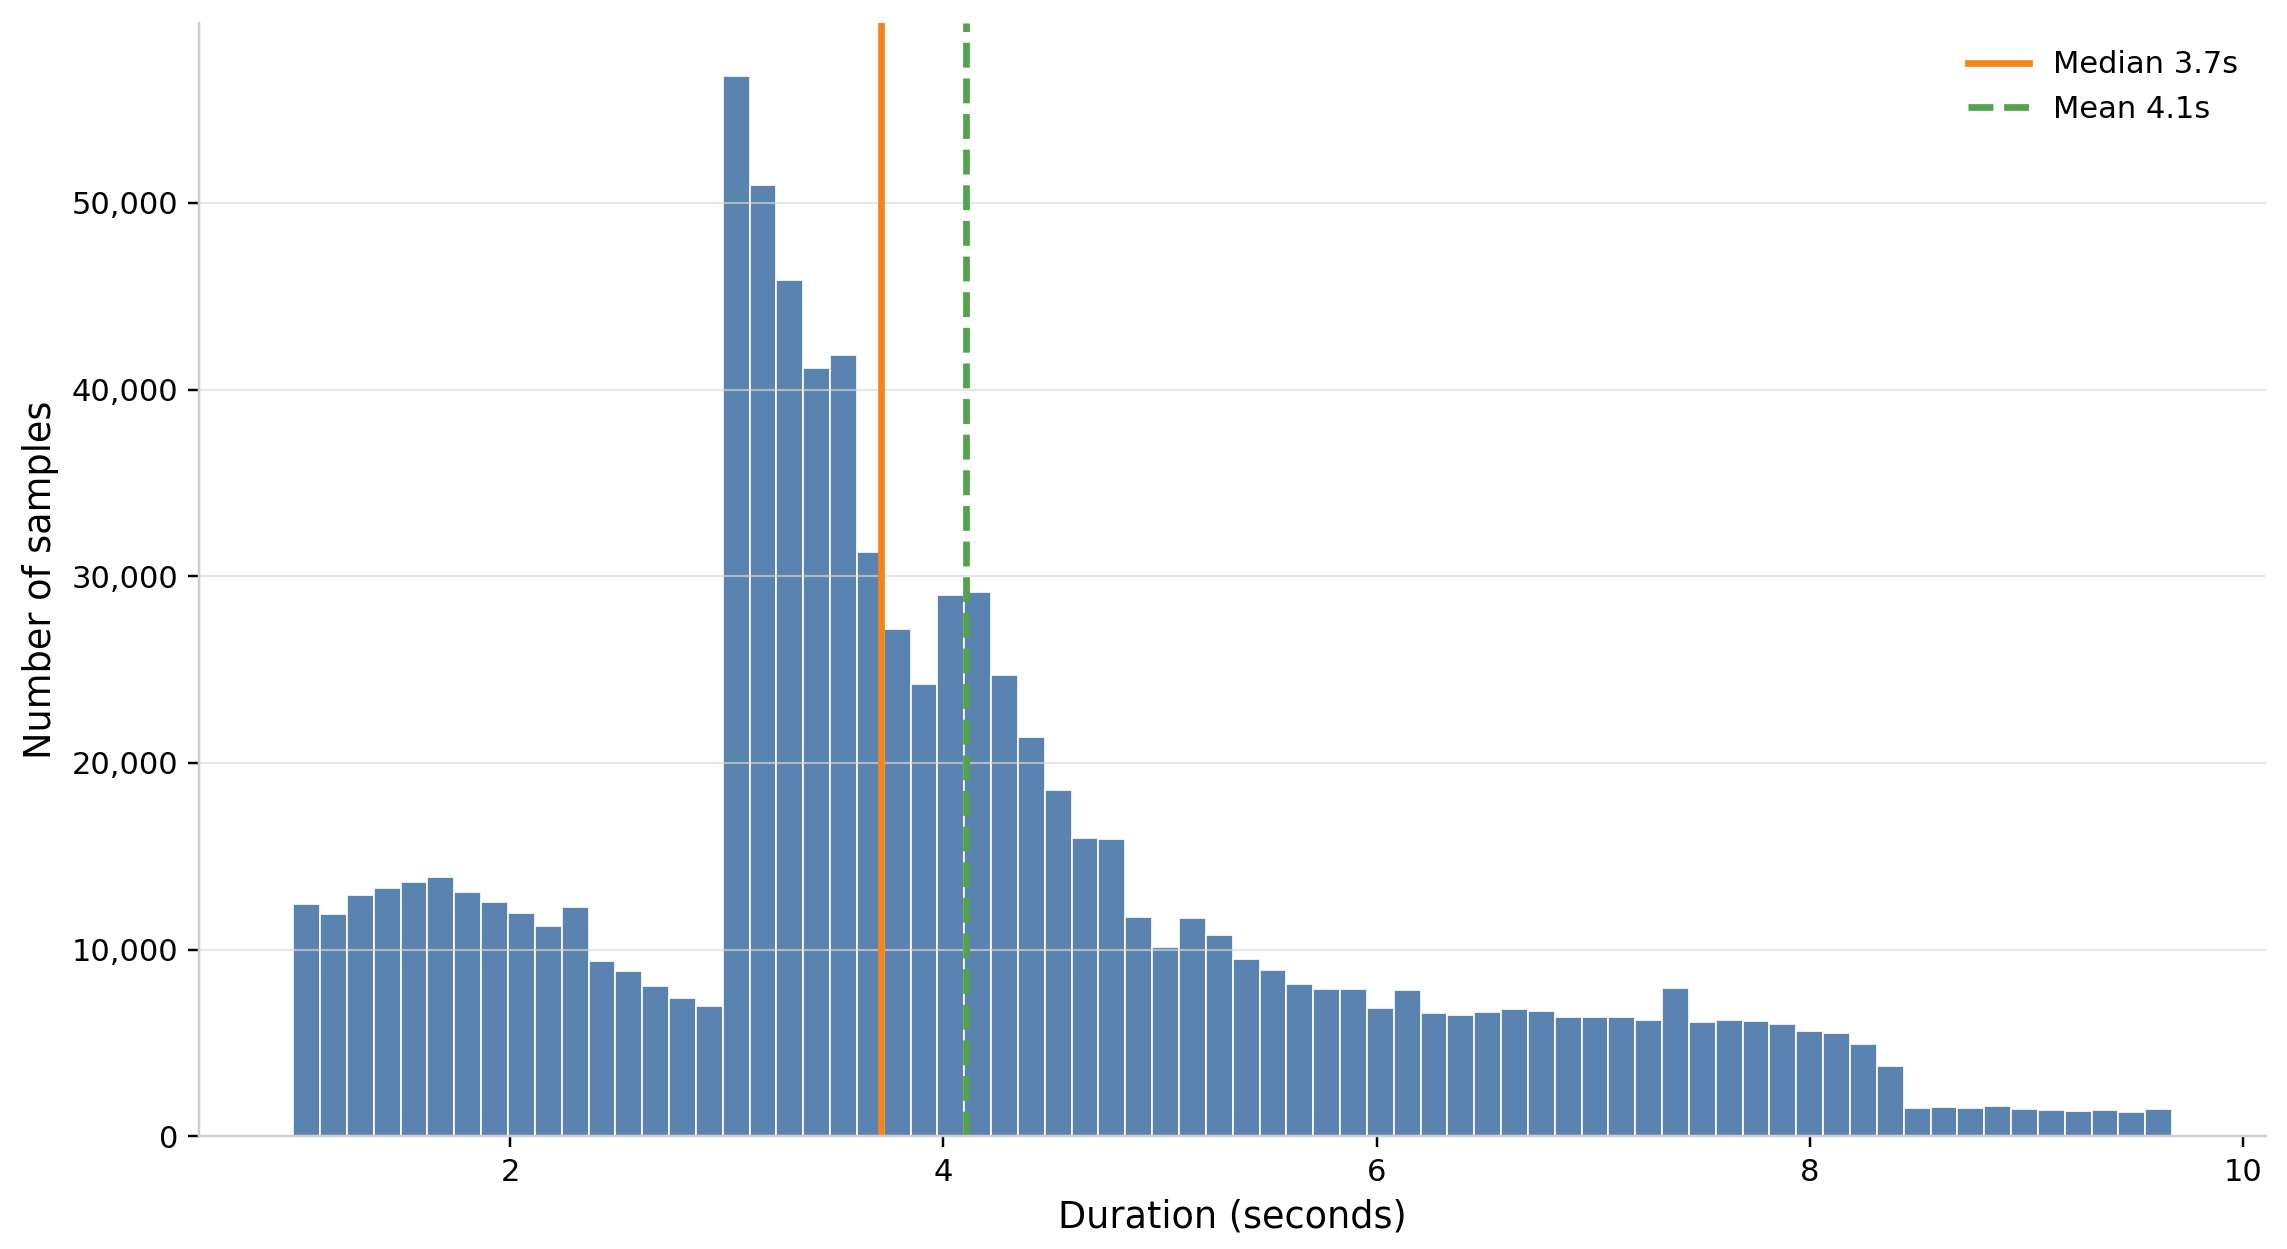
\includegraphics[width=0.9\columnwidth]{images/duration_hist.png}
\caption{Duration distribution of the curated training corpus.}
\label{fig:data_dur}
\end{figure}


\subsection{Data Labeling and Adjudication Pipeline}

% TODO: convert to TikZ flow diagram — domain-constraints.mdc §9
\begin{figure}[ht]
\centering
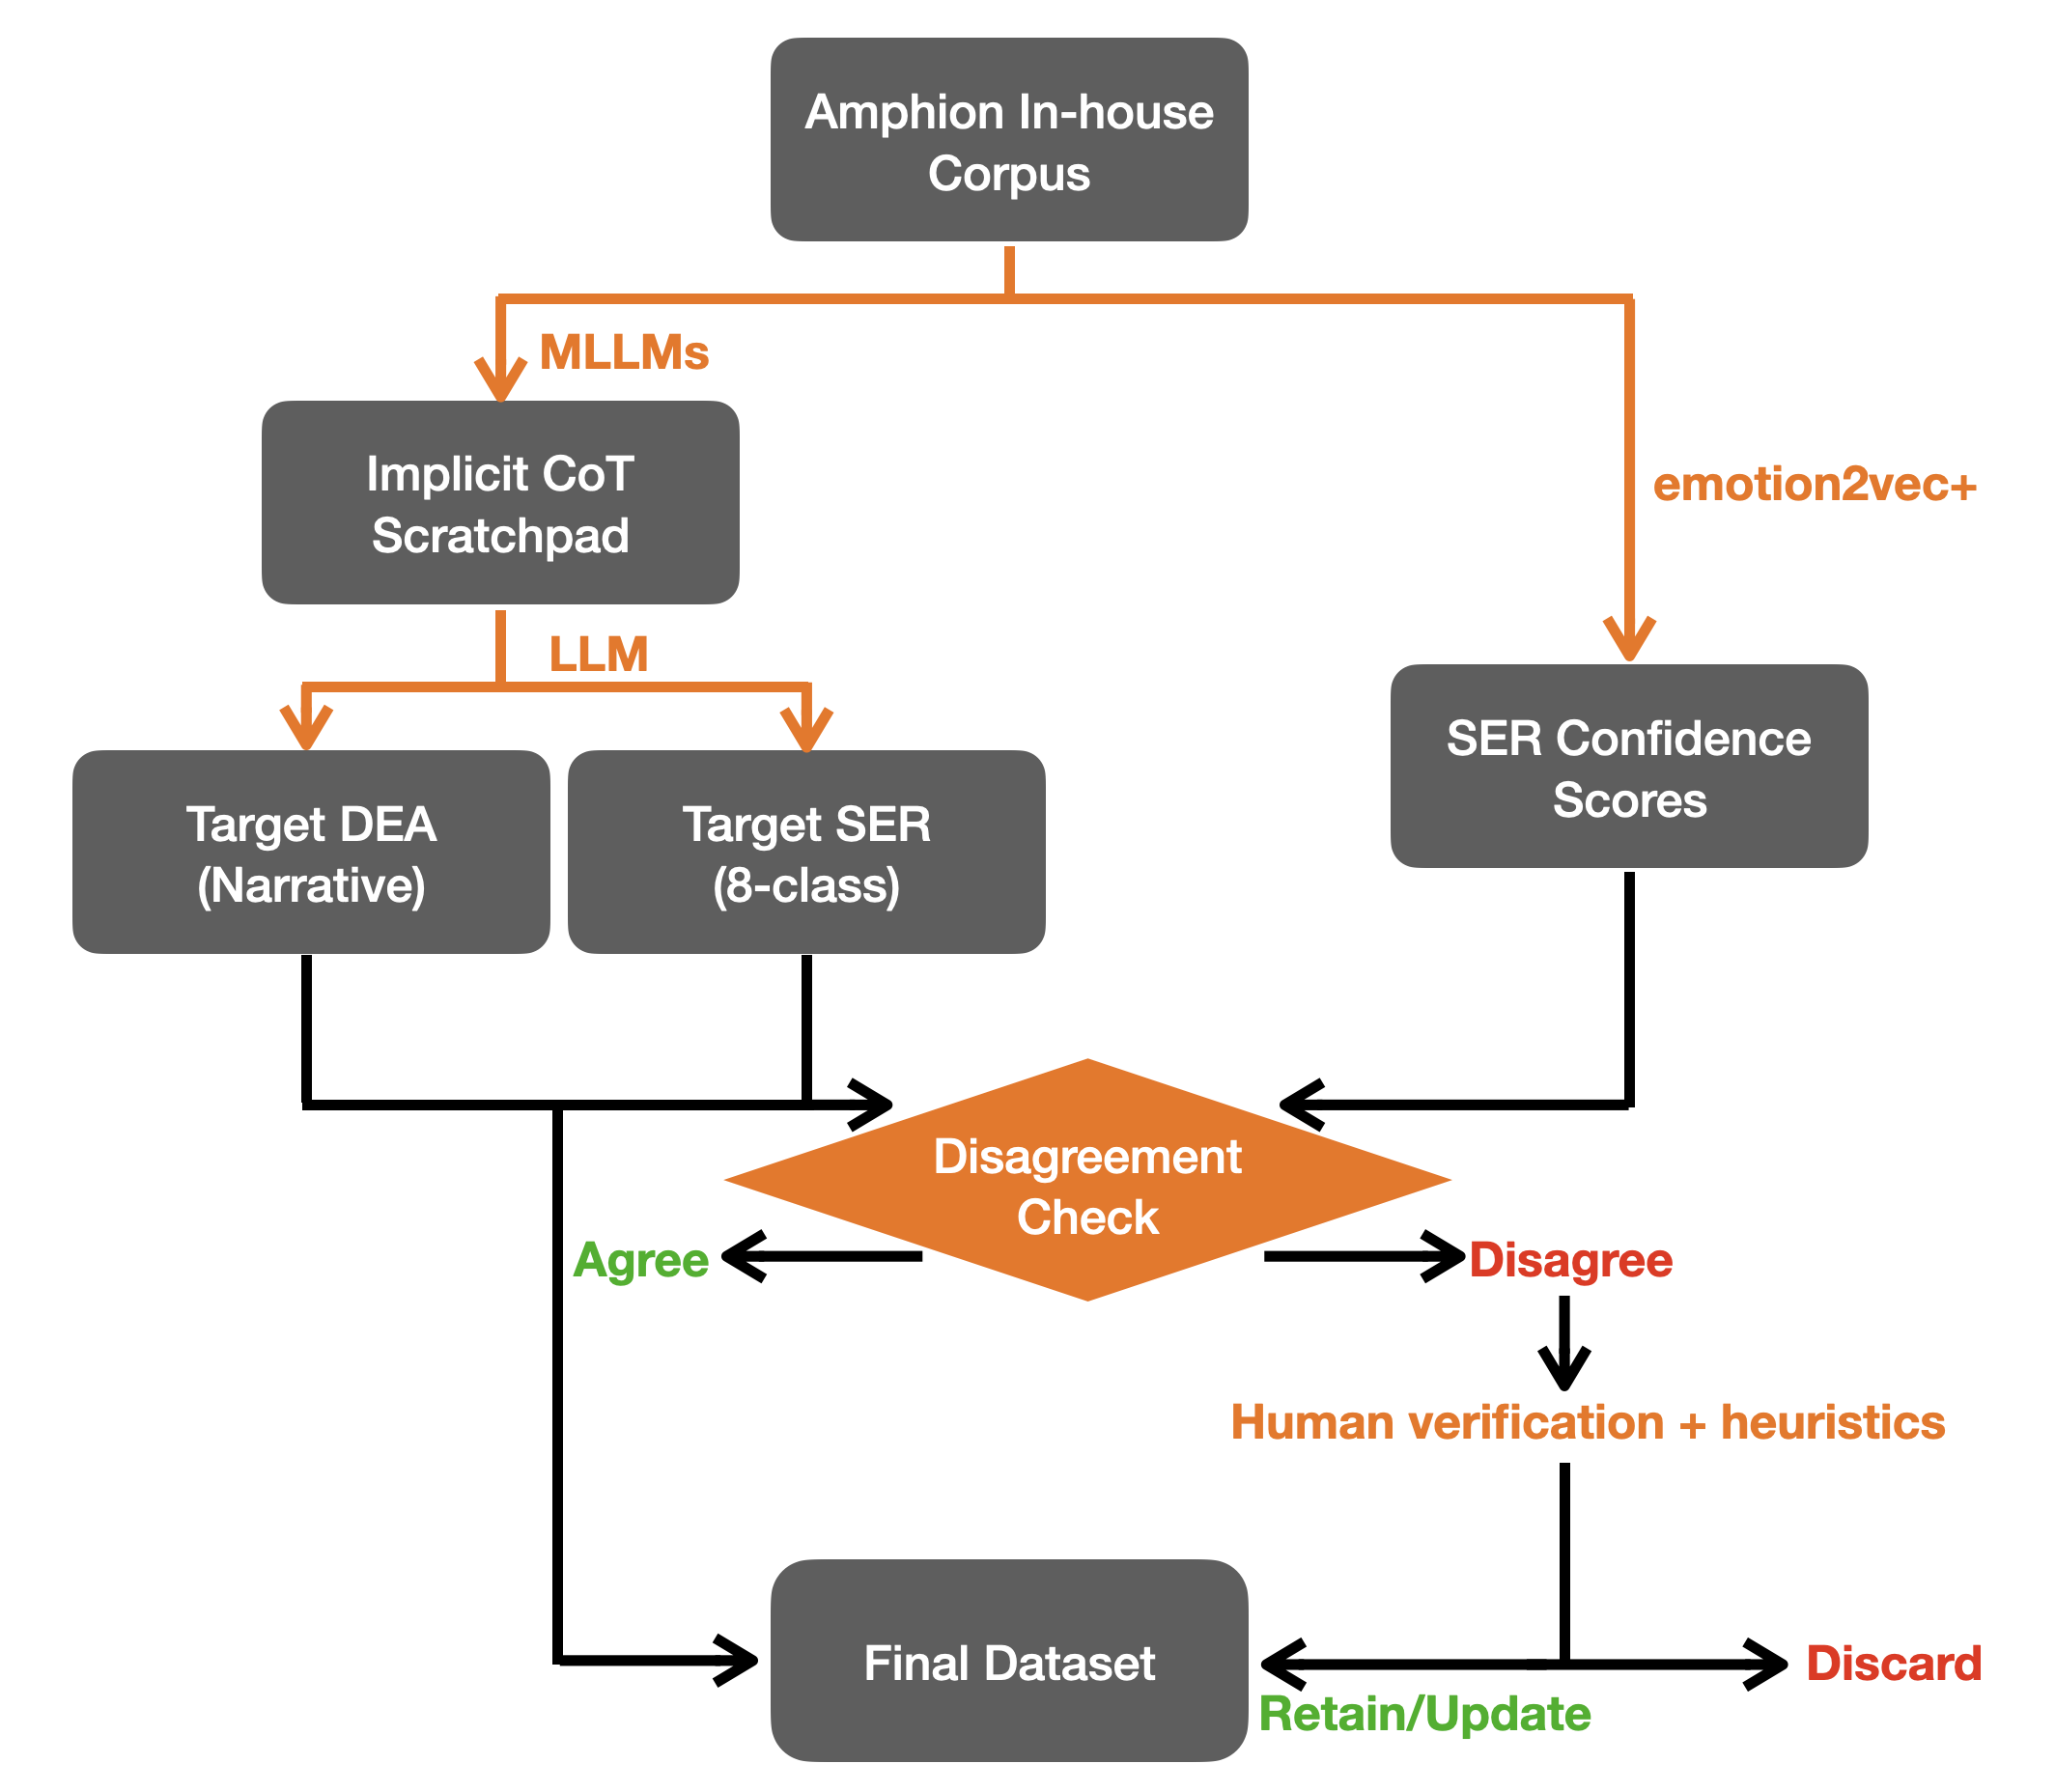
\includegraphics[width=0.7\columnwidth]{images/data_label_diagram.png}
\caption{Overview of the multi-stage data labeling and adjudication pipeline.}
\label{fig:data_label_pipeline}
\end{figure}

To annotate our large-scale audio corpus with high fidelity, we implemented a multi-model annotation pipeline leveraging state-of-the-art multimodal large language models (MLLMs), including Gemini~3.0~Flash \cite{gemini3} and GPT-4o \cite{GPT-4o}. Direct zero-shot classification of emotion from audio is particularly susceptible to a specific failure mode: MLLMs tend to assign emotion labels based on the \textit{semantic content} of the utterance (whether what is said sounds sad) rather than on the \textit{acoustic signal} (whether the delivery is breathy, tense, or hesitant). A sentence such as ``I'm completely fine'' may carry genuine neutrality, suppressed anger, or masked grief---three states that share identical lexical content but differ profoundly in their acoustic realization. To counteract this semantic-acoustic confusion, we mitigated this risk with structured decomposition prompting, inspired by Chain-of-Thought (CoT) reasoning \cite{CoT}: by requiring the model to first produce an explicit acoustic profile before committing to a label, we force attention to the perceptual rather than the semantic evidence.

Drawing on principles of decomposed prompting \cite{khot2022decomposed}, the MLLMs were instructed to avoid immediate classification. Instead, acting as expert auditory linguists processing the audio streams, they generated a multi-dimensional profile of the speech. This prompted the models to document speaker characteristics, prosodic rhythms, subtle paralinguistic shifts, and specific non-verbal vocalizations (NVVs) before drawing conclusions. The resulting profiles provided a rich perceptual foundation for downstream label extraction.

The natural language profiles generated during this decomposition stage acted as analytical scratchpads. In the subsequent step of the pipeline, we employed text-based LLMs to parse this dense textual analysis and distill the data into two target fields designed to support complementary downstream applications:
\begin{itemize}
    \item Standardized speech emotion recognition (SER): A definitive primary emotion classification restricted to a closed set of eight categories (happy, sad, neutral, angry, disgust, fear, surprise, and other/complex). This formulation ensures strict taxonomic alignment with established human-annotated datasets and our specialized expert model schema.
    \item Descriptive emotion analysis (DEA): A natural language speech description that goes beyond templated paralinguistic tags. While recent advancements such as SpeechCraft \cite{SpeechCraft} and ParaSpeechCaps \cite{ParaSpeechCaps} introduced valuable paralinguistic captioning, they rely on fixed or semi-fixed templated structures that constrain linguistic variance. Our extraction approach instead synthesizes cohesive narratives that integrate speaker attributes (\eg timbre, demographic traces), prosodic patterns, temporal emotional shifts, speech rate, and non-verbal vocalizations. This format is designed to capture complex auditory nuance for downstream generative tasks and advanced audio-language reasoning.
\end{itemize}

To increase confidence in these extracted labels, we paired the MLLM pipeline with a targeted human-in-the-loop verification protocol driven by a specialized categorical expert model. We deployed emotion2vec+ \cite{emotion2vec}, a dedicated architecture for speech emotion recognition, to independently process the raw audio and compute confidence scores (normalized probability distributions) across the eight SER categories.

Our automated pipeline cross-referenced the primary SER classification extracted from the highly perceptive MLLMs against the categorical probabilities computed by emotion2vec+. Any samples exhibiting a high-confidence disagreement---specifically, instances where the MLLM's chosen emotion corresponded to a strictly low probability score from the emotion2vec+ verification model---were automatically flagged as complex edge cases. We subsequently isolated a random subset of these contested instances for manual investigation by human experts.

By analyzing the root causes of these model divergences---such as sarcasm, bilingual code-switching, or multi-tonal speech---we formulated deterministic, heuristic rules. These rules dictated the systematic retention, correction, or rejection of the complete annotation suite for conflicting samples. This meant curating not only the discrete SER labels but also refining or discarding the associated descriptive emotion analysis (DEA) narratives when the models failed to align. By pruning low-confidence annotations and enforcing consistency between categorical labels and descriptive narratives, the pipeline produced a more reliable and internally consistent training corpus.

% TODO: convert to pgfplots bar chart (requires per-category count data) — domain-constraints.mdc §9
\begin{figure}[ht]
\centering
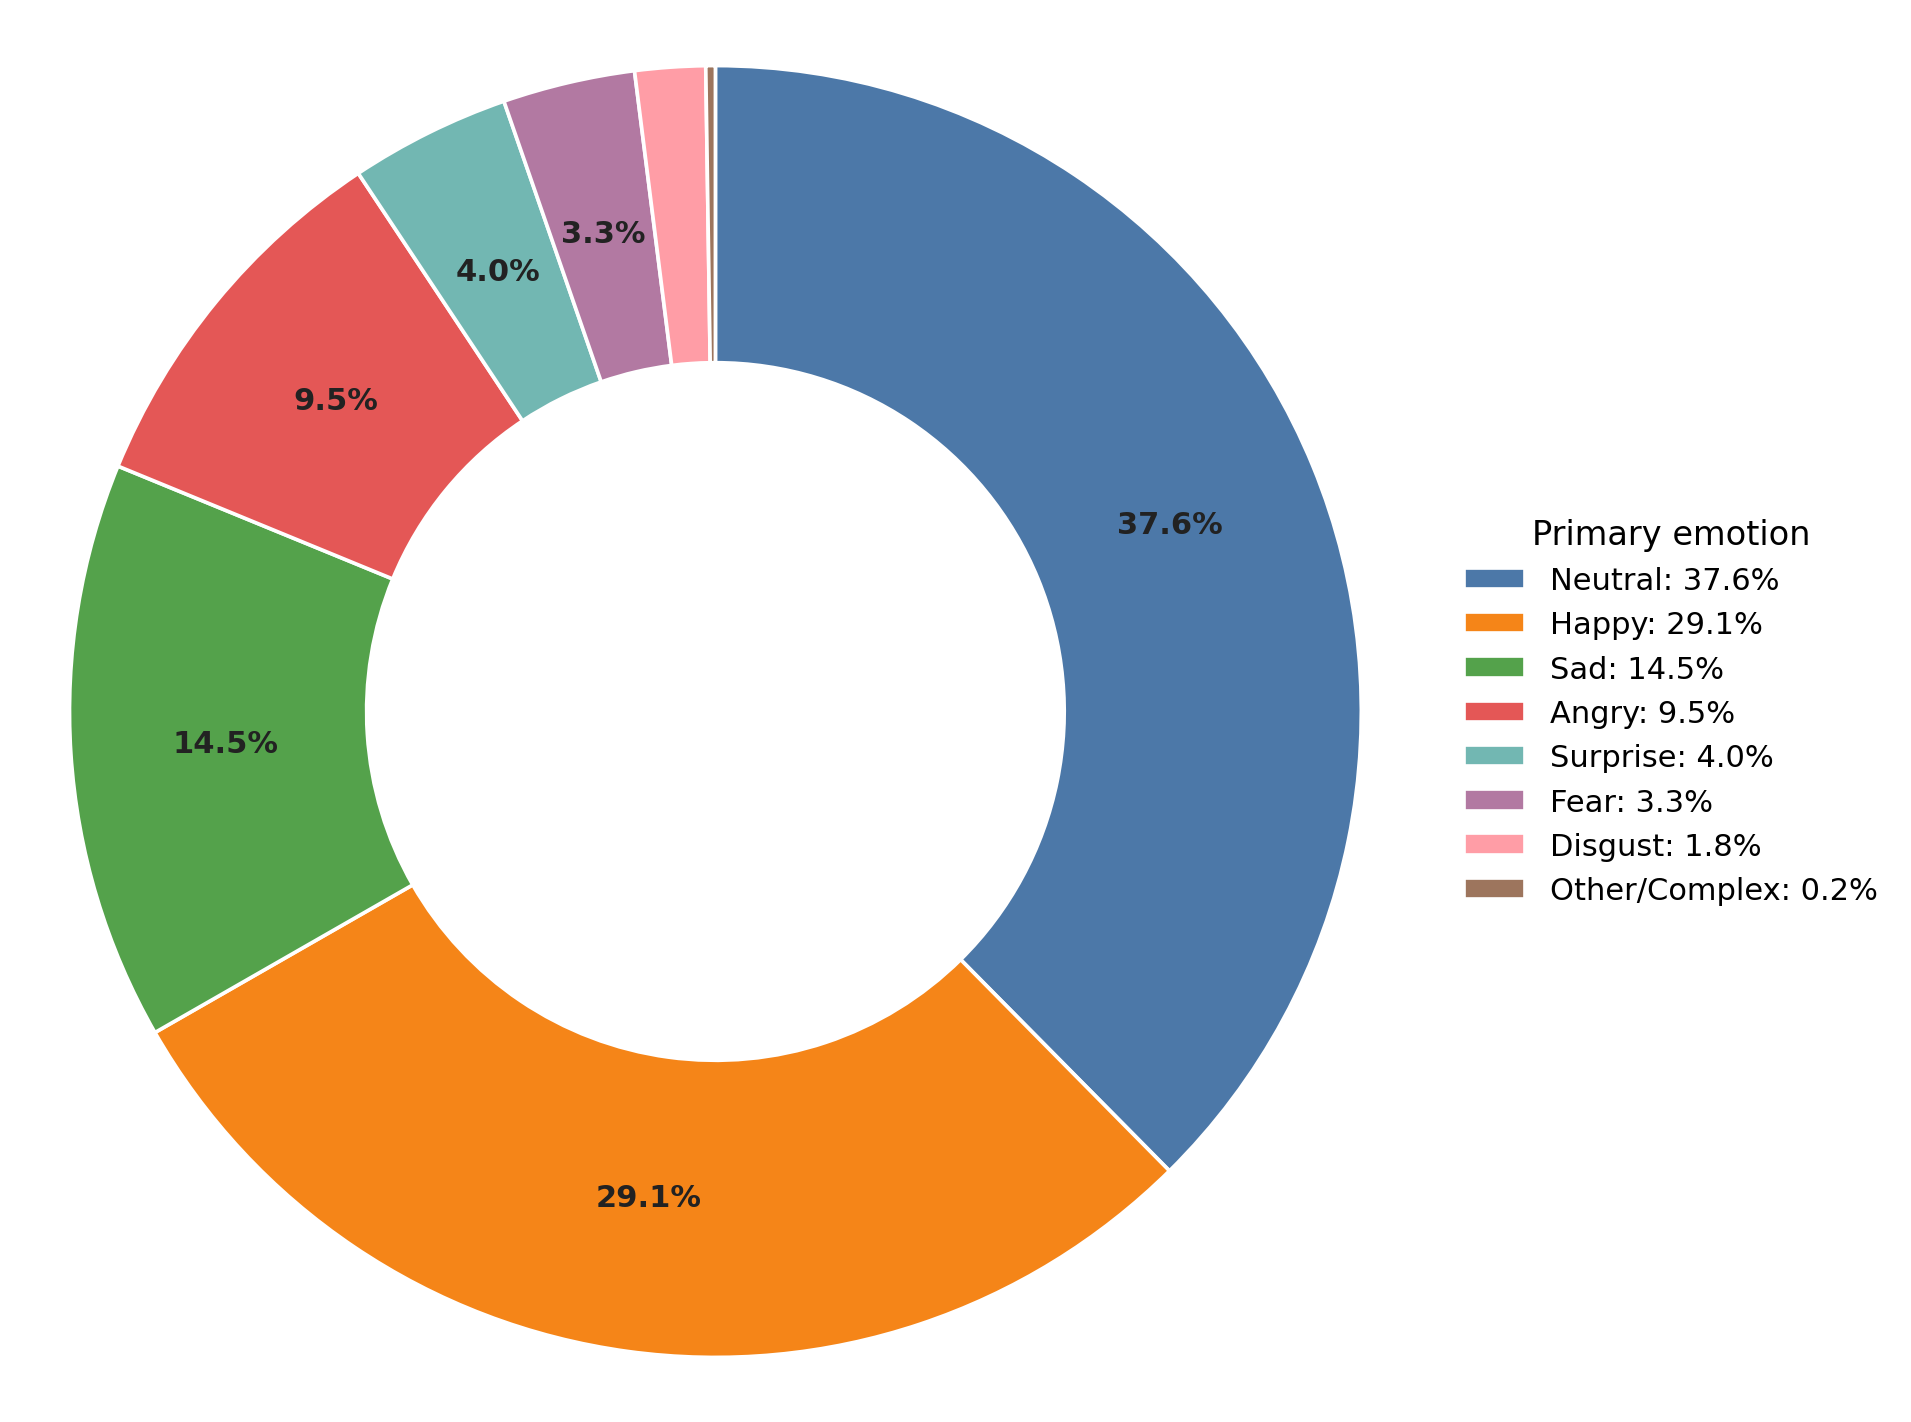
\includegraphics[width=0.6\columnwidth]{images/primary_emotion_dist.png}
\caption{Primary emotion distribution of the curated corpus. Chinese and English subsets share roughly the same distribution.}
\label{fig:primary_emotion_dist}
\end{figure}
